\chapter{Knowledge Distillation}
\label{part_2}
\acrfull{kd} is a frugal AI technique known to provide great results. Using the results of a large model at training time, a smaller model can achieve performances which tends towards that of the large model. This chapter focuses on applying \acrshort{kd} to \acrshort{lic}. In order to do that, we first experiment with \acrshort{kd} on auto-encoders for image reconstruction. After achieving satisfactory results, we proceed in implementing \acrshort{kd} for \acrshort{lic}.

\section{Knowledge Distillation for Auto-encoders}
% Image reconstruction is similar but simpler than lic
As explained by Ballé et al. in \cite{ballé2018variationalimagecompressionscale}, \acrshort{vae}s are very similar to \acrshort{lic} architectures in the sense that they both have some sort of analysis transformation to transfer the input signal to a low dimensional latent space and an approximate of this analysis transform (the synthesis transform) to transfer the latent representation back to the signal space. However, in \cite{minnen2018jointautoregressivehierarchicalpriors}, the authors explain the difference between the two. Compression consists in reducing the entropy of the representation under a prior probability model shared between the sender and the receiver, not only the dimensionality. Achieving performant image compression/decompression is thus more complex than doing standard image reconstruction.

In the context of this study, applying \acrshort{kd} to auto-encoders for image reconstruction is a step in the right direction as it is a similar yet easier task than image compression. First, we become acquainted with this technique by implementing it on custom made \acrshort{ae}s. Following that, we apply the same technique to state-of-the-art image compression models used as \acrshort{ae}s.

\subsection{Custom Auto-encoder}
The goals of this experiment are straightforward: experimenting \acrshort{kd} on known architectures such as convolutional \acrshort{ae} and assessing the effect of \acrshort{kd}. To do so, we train a large model (the teacher model) and a small model with and without \acrshort{kd}. We expect the model trained with \acrshort{kd} (the student model) to achieve better image reconstruction performance than the other small model. In the best case scenario, the student model would give results similar to that of the teacher model.

We design the teacher encoder with three stages each containing two convolutions with ReLU followed by a maximum pooling. This is followed by a two-layer fully connected network to achieve a latent space size of 256. The teacher decoder follows the same structure but reversed with transpose convolutions instead of convolutions and up-sampling to replace pooling. The small architecture is analogous with only one convolution (or transpose convolution) per stage.

[TODO: retrain + results]

An interesting experiment to perform would be to create another student architecture with the same encoder as the teacher and only a smaller decoder. This set-up would fit more the context of image compression with a single sender that compresses the image with a powerful encoder and multiple resource constrained receivers using an efficient decoder.

\subsection{Scale Hyperprior Model as Auto-encoder}
With the previous section showing the benefits of \acrshort{kd} for auto-encoders, the hope for this technique to work for image compression increased. Following a step-by-step approach, we first tried to observe similar results with the architectures used for image compression. The goal of the following experiment is to use the state-of-the-art scale hyperprior model as an auto-encoder for image reconstruction. As discussed previously, image reconstruction is very similar to image compression but with no entropy constrain on the latent space. The scale hyperprior model, designed for \acrshort{lic} should reach satisfactory performances on this easier task. The additional benefit of this experiment being that the code used will form a foundation for future experiments focused on \acrshort{lic}.

% Optional: KD from scratch...

Now that we are familiar with \acrshort{kd}, we should highlight the importance of the "quality" of the teacher. If we continue the analogy of the teacher and student relationship, it makes sense that a good teacher is more likely to train a good student than a bad teacher. This principle can be applied to \acrshort{kd}. As the student learns partially from the output of the teacher, we must use a powerful teacher network, otherwise the student network will learn poor latent representations as well as reconstructions. In order to achieve the best possible results, we decided to perform the upcoming experiments using pre-trained networks from the compressAI model zoo as teachers. On top of dramatically reducing hte training time fro each experiment, it also allow us to easily compare our models to state-ot-the-art results.

% Explain why number of channels next???

The following experiment consists in training five students models with different architectures. Using the pre-trained scale hyperprior model optimised for MSE with \textsf{quality} set to 5 (which corresponds to 128 channels and a latant space of size 192), we experiment with models with different number of channels. We define five models with 16, 32, 64, 96 and 112 channels while preserving the size of the latent space. We use the following \acrshort{kd} loss function:

\[L = \lambda_{1} MSE(z_{student}, z_{teacher}) + \lambda_{2} MSE(\hat{x}_{student}, \hat{x}_{teacher}) + \lambda_{3} MSE(\hat{x}_{student}, x)\]

We use the following parameters: \(\lambda_{1} = 0.2\), \(\lambda_{2} = 0.2\), \(\lambda_{3} = 0.6\) and train the models with the same methodology as in Chapter \ref{part_1}, meaning: 1000 epochs on the Vimeo90K dataset with a base learning rate of \(10^{-4}\).

Figure \ref{kd_ae_1:a} shows reconstructions of image 14 of the Kodak dataset with the teacher and all student networks. As axpected, the teacher (a pre-trained model) propose a reconstructed image virtually undistinguishable from the orignal one. As for the students, eventhough they give visually satisfying results, the models with less parameters do not retain as much details. The reconstructed image appears a little bit blurry. As expected, the more the student architecture is similar to the teacher (that is to say, larger), the more it is able to reach the same performance as the teacher. This is quantitatively measured using MSE on Figure \ref{kd_ae_1:b}.

\begin{figure}[H]
    \centering
    \subfloat[Reconstruction results on image 14 of the Kodak dataset with teacher and student architectures.]{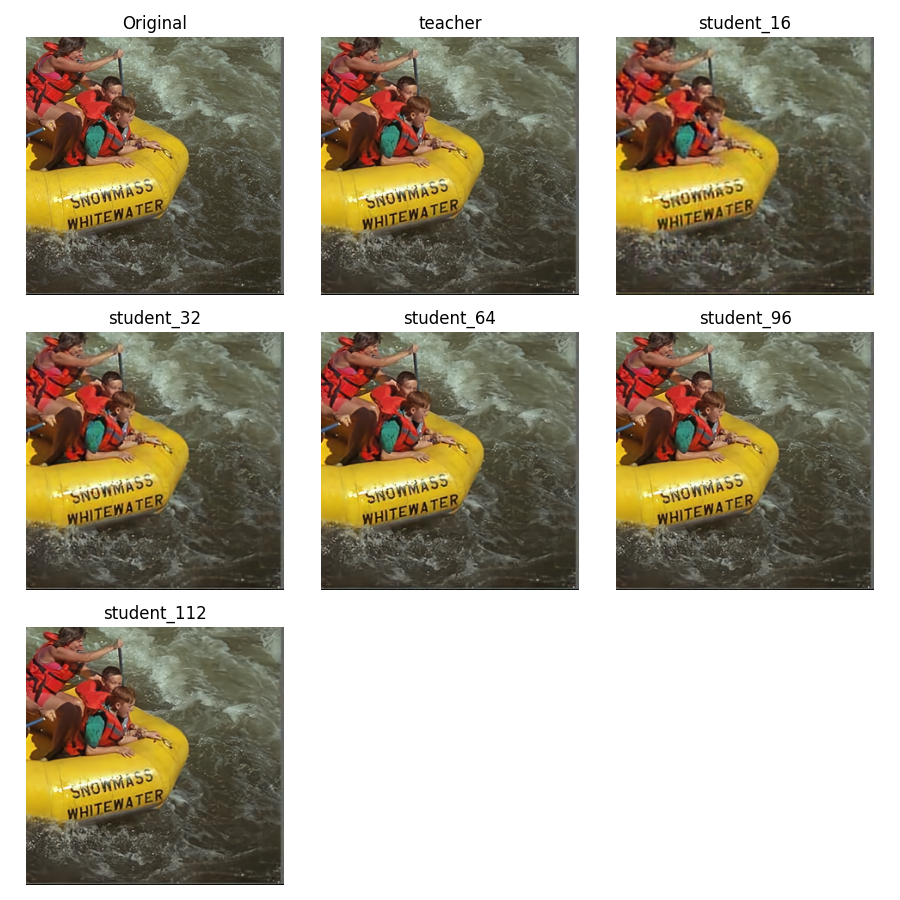
\includegraphics[width=8cm]{img/kd_ae_1.png} \label{kd_ae_1:a}}
    \qquad
    \subfloat[Pre-trained networks]{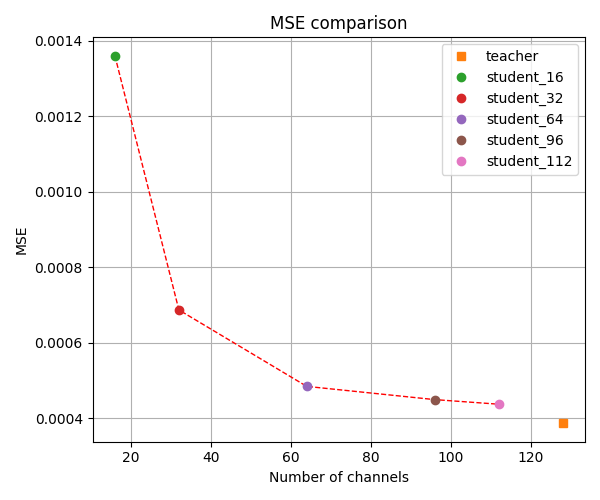
\includegraphics[width=8cm]{img/kd_ae_2.png} \label{kd_ae_1:b}}
    \caption[]{}
    \label{kd_ae_1}
\end{figure}

For reference, we show in Figure \ref{kd_ae_2} the \acrshort{rd} performances of the student models. It should be noted that the teacher network used in this experiment was trained for image compression tasks. One could argue that these models are not exactly auto-encoders for image reconstruction. What is sure is that they are far from state-of-the-art models in image compression tasks. What remains to be seen is to what extent a properly defined \acrshort{kd} loss for \acrshort{lic} does increase the \acrshort{rd} performance of these student models. This, as well as discussion related to the benefits of smaller student models for \acrshort{lic}, is the subject of the next section.

\begin{figure}
    \centering
    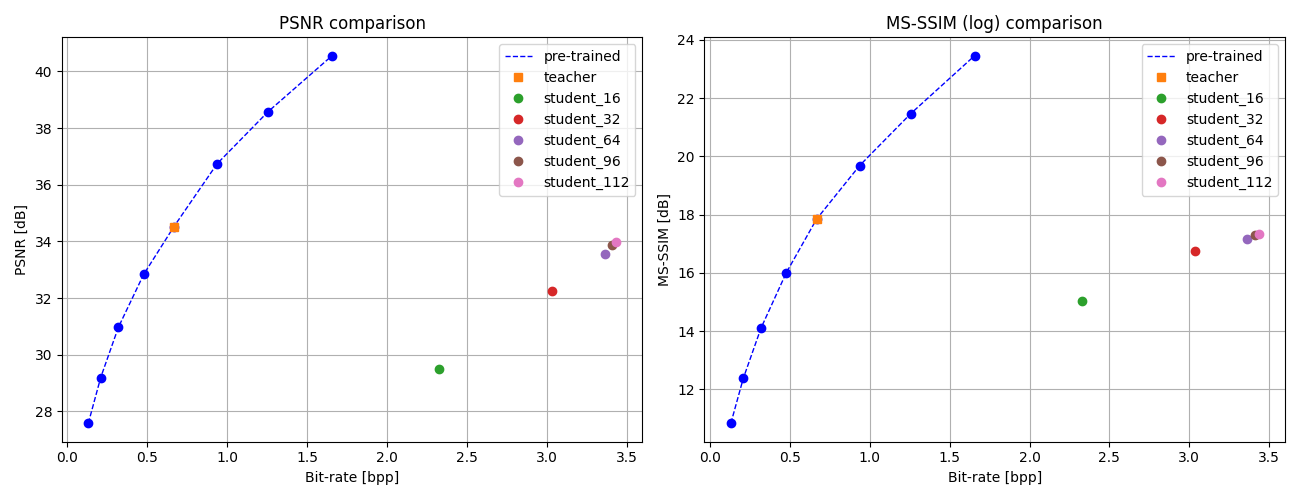
\includegraphics[width=15cm]{img/kd_ae_3.png}
    \caption[]{}
    \label{kd_ae_2}
\end{figure}

\section{Knowledge Distillation for Image Compression}
% Eventhough similar image reconstruction is different than image compression which requires min entropy
Our work on this topic can be summarised as follow: ...
